\chapter{Introduction}

\section{Section}\label{sec:example}
\subsection{Subsection}\label{sec:example2}
\subsubsection{Subsubsection}


\charef{cha:conclusion}

\appref{app:example}

\secref{sec:example}

\secref{sec:example2}

\section{Figures}

\begin{figure}[ht]
\centering 

\includegraphics[scale=0.4]{Figures/jpgFigure.jpg}
\caption{JPG figure title.}
\label{fig:jpgFigure}
\end{figure}

\begin{figure}[ht]
\centering 
\subfigure[PDF figure title.]{
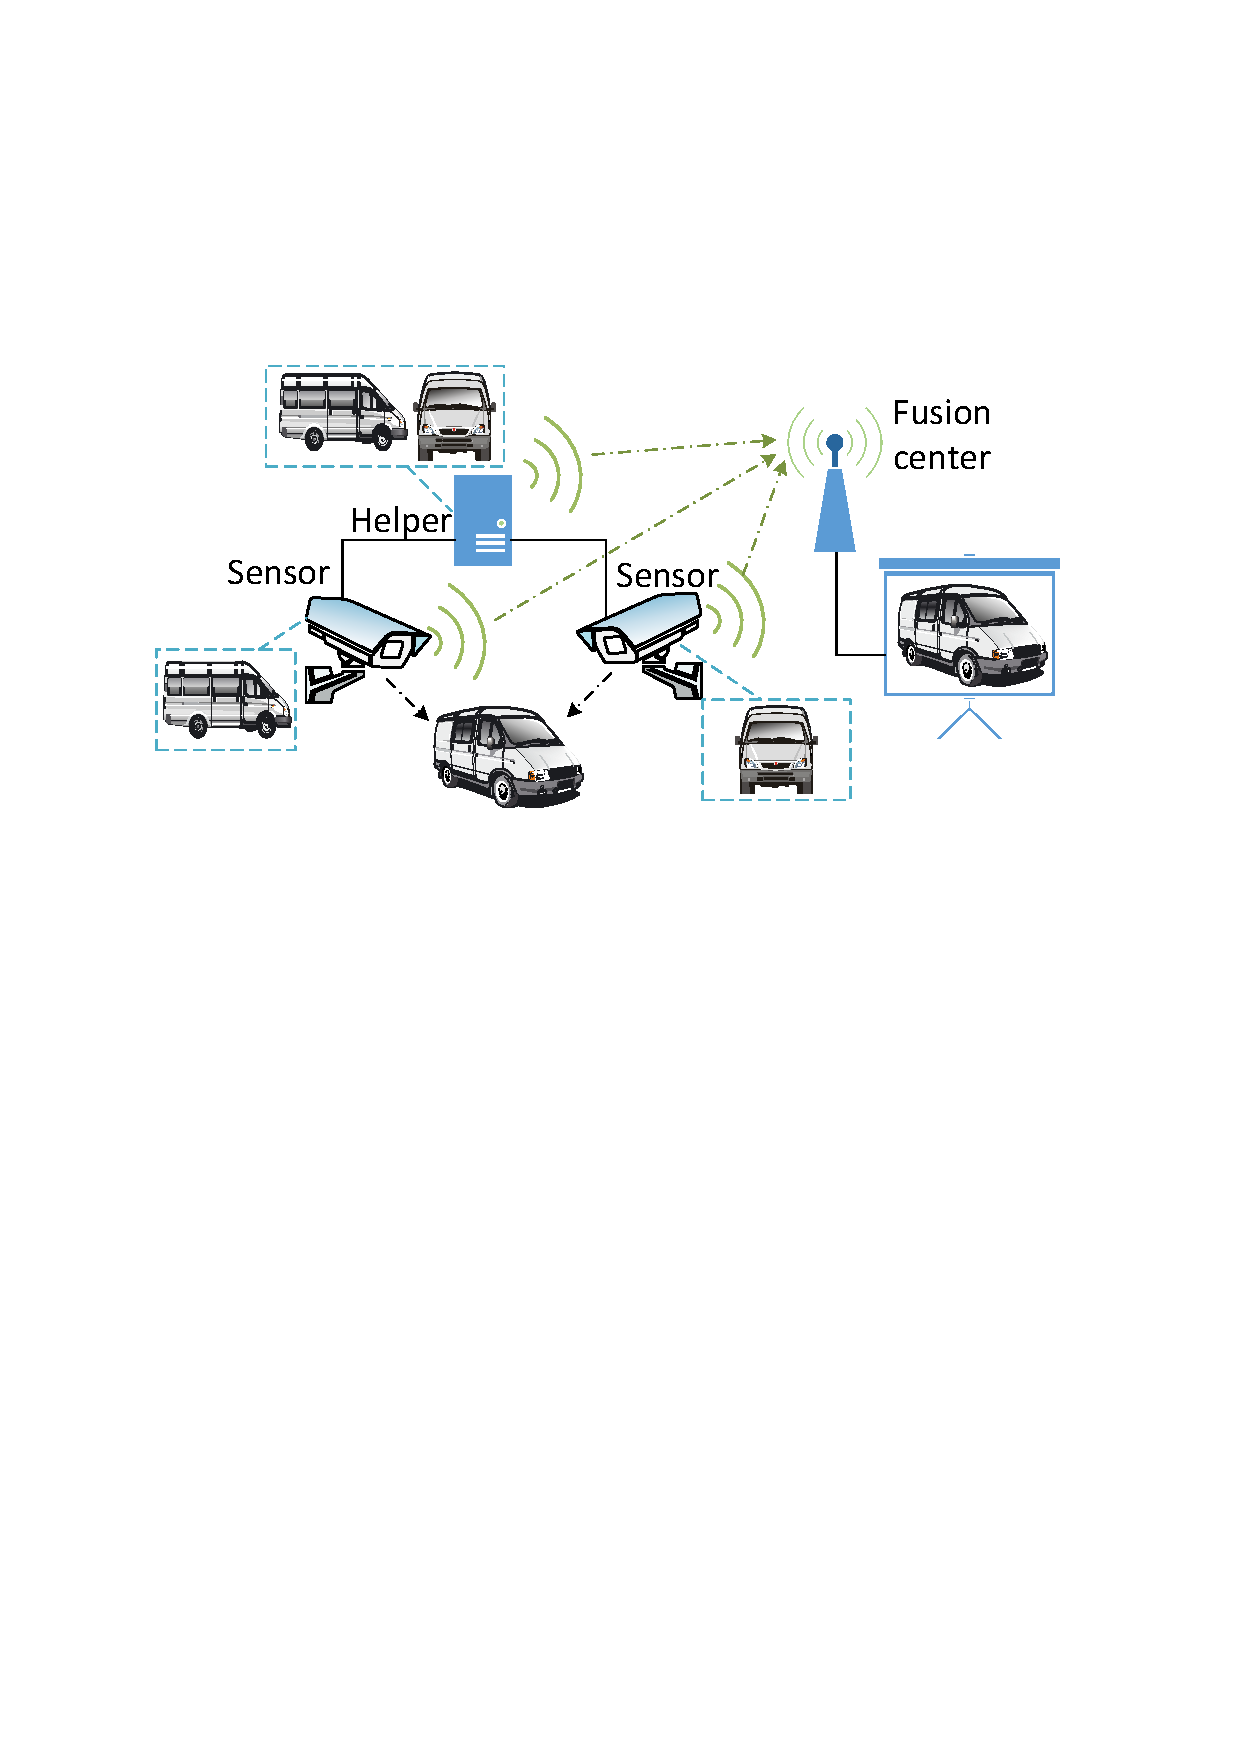
\includegraphics[height=4cm]{Figures/pdfFigure.pdf}
\label{fig:pdfFigure}
}
\subfigure[EPS figure title.]{
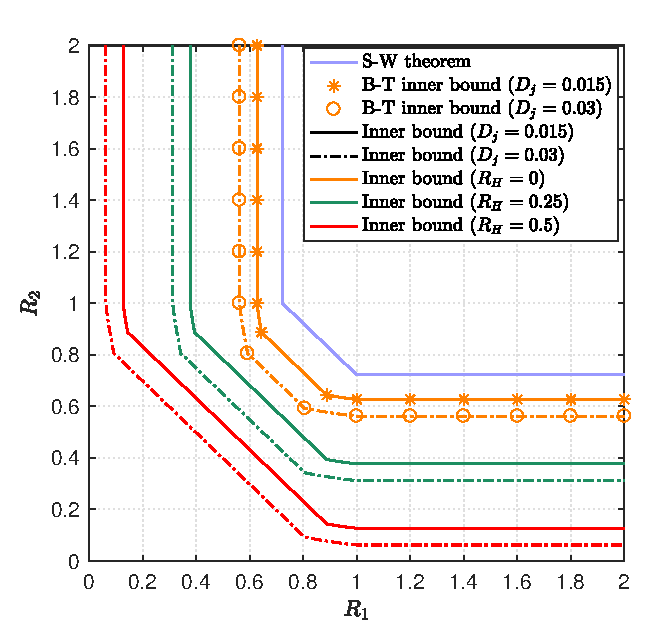
\includegraphics[height=4cm]{Figures/epsFigure.eps}
\label{fig:epsFigure}
}
\caption{Subfigure Examples.}
\label{fig:examples}
\end{figure}

\fref{fig:jpgFigure}

\fref{fig:examples}

\fref{fig:epsFigure}

\section{Tables}
\begin{table}[ht]
\centering
\begin{tabular}{m{1cm}|rr}
& a & b\\ 
\hline
1& 0.25 & 0.33\\
2& 0.75 & 0.66\\
\end{tabular}
\caption{Caption of the table}\label{table:example}
\end{table}

\tref{table:example}

\section{Equations}

\begin{equation}
x = \frac{-b \pm \sqrt{b^2-4ac}}{2a}. \label{eq:example}
\end{equation}

\begin{align}
x^2 &= -(2x +1) \\
x^2 &= -2x -1 \nonumber\\
x^2+2x +1 &= 0 \label{eq:example2}\\
(x+1)^2 &=0 \label{eq:example3}.
\end{align}

\eqref{eq:example3}

\eqsref{eq:example}{eq:example2}

\section{Abbreviations and Symbols}
\gls{iid}


\Gls{CEO}


\glspl{CEO}

\gls{IoT}


\Glspl{pmf}

\section{Citations}
\cite{berger1978multiterminal}

\cite{berrou1996near,shannon1959coding,el2011network,mp3standard}

\cite{el2011network,berger1978multiterminal}

\cite{Tung1978multiterminal}

\section{Algorithms}
\begin{algorithm}
\caption{An Example}
\label{alg:example}
\begin{algorithmic}
\REQUIRE {$x$, $n$} 
\ENSURE {$y$}
\STATE {set $y=1$;} 

\IF	{$n==0$} 
	\STATE {set $y=1$;} 
\ELSIF {$n>0$} 	
	\FOR {$i=1$ \TO $n$} 		
		\STATE {set $y = y \times x$;} 
	\ENDFOR
\ELSE
	\FOR {$i=n$ \TO $-1$} 		
		\STATE {set $y = y \div x$;} 
	\ENDFOR 
\ENDIF
\end{algorithmic}
\end{algorithm}

\algref{alg:example}

\section{Codes}
\begin{lstlisting}[
	language=C++,
	title={No Number Title},
	label={code:example} ] % 设置语言、标题、标签
%以下插入代码,必须隔一行空行

int main(){
	for(int i=0; i<3; i++){
		cout<<i<<endl;
	}
	return 0;
}
\end{lstlisting}

\lstinputlisting[
	language=TeX,
	caption={Input Code from File},
	label={code:input}]
	{Chapters/Conclusion.tex} %从文件中插入代码

\coderef{code:input}

\subsection{Definition, Lemma, and Proposition}

\Definition\label{def:example} Example Definition

\Lemma\label{lem:example} Example Lemma

\Proposition\label{pro:example} Example Proposition

\ref{def:example}

\ref{lem:example}

\ref{pro:example}